\documentclass{article} % For LaTeX2e
\usepackage{nips15submit_e,times}
\usepackage{hyperref}
\usepackage{url}
\usepackage{graphicx}
%\documentstyle[nips14submit_09,times,art10]{article} % For LaTeX 2.09


\title{CS522 - Prediction of Grant Applications}


\author{
Priyaranjan Behera\\
Department of Computer Science\\
North Carolina State University\\
\texttt{pbehera@ncsu.edu} \\
\And
Sai Sri Harsha Kunapareddy\\
Department of Computer Science\\
North Carolina State University\\
\texttt{skunapa@ncsu.edu} \\
}

% The \author macro works with any number of authors. There are two commands
% used to separate the names and addresses of multiple authors: \And and \AND.
%
% Using \And between authors leaves it to \LaTeX{} to determine where to break
% the lines. Using \AND forces a linebreak at that point. So, if \LaTeX{}
% puts 3 of 4 authors names on the first line, and the last on the second
% line, try using \AND instead of \And before the third author name.

\newcommand{\fix}{\marginpar{FIX}}
\newcommand{\new}{\marginpar{NEW}}

\nipsfinalcopy % Uncomment for camera-ready version

\begin{document}


\maketitle

\begin{abstract}
There is a relative shrinking of the pool of funds available to people in academia to pursue research. The diminishing success rates mean academics spend their valuable time on applications which will end up being rejected. To address this, University of Melbourne hosted a kaggle competition to develop methods to predict the outcomes of the grant applications. 

This project focuses on finding an accurate method to predict grant applications. We are applying methodologies like Decision Trees, Bagged and Boosted Trees, Neural Network, SVM to build models for the prediction and compare the models based on the problem specifications to come out with the most efficient model. 
\end{abstract}

\section{Background}

Around the world, the pool of funds available for research grants is steadily shrinking (in a relative sense). In Australia, success rates have fallen to 20-25 per cent, meaning that most academics are spending valuable time making applications that end up being rejected. This problem was hosted as a competition by University of Melbourne to address their inefficiencies with the grant applications. There is also a hope of discovering the most important criteria that are required to succeed in a grant application. 

\subsection{Problem}

The university has provided a dataset containing 249 features, including variables that represent the size of the grant, the general area of study and de-identified information on the investigators who are applying for the grant. The dataset contains multi-variate data with a few of them being continuous variable and a few categorical. There is a variable number of investigators in an application and thus, we need to aggregate the person data to create an efficient model. We are looking into implementing several of the classification techniques covered in the CS522 course to arrive upon an efficient model.


\subsection{Literature Survey}

The dataset contains a variable number of person attributes for each of the investigators in an grant application. This would lead to multiple missing data fields in applications where the investigator count is less. According to Gerhard Svolba \cite{OneRow}, we need to create a one-row-per-subject data mart for most of the analytical methods that we need to proceed with. Accordingly, we need to aggregate the person data using mean, median, standard deviation, the quartiles, or special quantiles, etc to create the input rows.

We looked at approaches taken to solve similar problems which contains both continuous and categorical data \cite{Matlab} and found that decision trees and naive bayes are popular choices. On the contrary, methods like neural networks, SVM, etc. cannot work with categorical data. We will be looking to implement decision trees as well as bagged and boosted trees for more efficiency. 

Daniele et al. \cite{HighCard} focused on the transformation of categorical data to continuous/binary data so that we can use the analytical methods which cannot process categorical data. While traditionally 1-to-n encoding is used for conversion of categorical data to binary, for categories with high cardinality a probabilistic approach is suggested.

\section{Methods}

The analysis of the data required extensive preprocessing steps because of its multi-variate nature and variable number of attributes. We look to implement different type of classification techniques to compare the models and find the determining attributes for the classification.

\subsection{Preprocessing}

To handle the categorical values in the data, we indexed the attributes with numerical values after finding the unique values for each of the attributes. As per the approach suggested by Gerhard Svolba \cite{OneRow}, we aggregated the person data for each of the application which is not null and found the minimum, maximum for all the attributes. While for continuous attributes we also calculated mean, median, sum of the values to create new features. We then created plots of the attributes with respect to the output to visually inspect any correlation of the attributes with the results.

Since many of the classification techniques cannot handle categorical data, we look to implement 1-to-n encoding to convert the categorical data into binary attributes which can be used in the analytical techniques. Further, to handle high cardinality, we will implement a probabilistic feature creation as specified at \cite{HighCard}. 

\subsection{Classification}

We look to implement most of the classification techniques covered in CS522 and compare their efficiencies.

\subsubsection{Decision Tree and Random Forest}
According to our survey of approaches employed for similar problems, decision tree turns out to be a popular choices. This is attributes to the fact the it can handle categorical values without any further processing. We also implement bagged trees using the dataset to get a more efficient classification. We also can use the decision tree to determine the most important factors which decides the success of a grant application.

\subsubsection{Neural Networks}
Since the neural networks can handle a high number of attributes, this will serve as an ideal classifier particularly when we use the 1-to-n encoding with a high cardinality of the categorical attributes. However, we cannot determine the determining factors of an application though this method.

\subsubsection{Naive Bayes}
Since categorical variables can also be handled by the Naive Bayes approach, we will use this classification method. However, we will extract the determining features by the use of the decision tree and use only a fraction of the features which has high effectiveness. 


\section{Plan}
According to the problem statement of the competition, we will be aiming to find a model which has a greater accuracy while minimizing the False Positives in the output.

\subsection{Hypothesis}
We will work on implementing models of the classifications techniques we have been familiarized with to find a model with lesser number of false negatives and higher accuracy. Thus, we will focus on the values of True Positive Rate, False Positive Rate, Precision and Accuracy of the models. Most importantly, we will be using the ROC (Receiver Operating Curve) to determine the effectiveness of the model by comparing the area under the curve for the models. This will be more helpful compared to other criteria as:
\begin{itemize}
	\item It is insensitive to unbalanced dataset where there is a disparity in the number of test cases outputs.  
	\item We consider all the cut-offs in a model to find its effectiveness.
\end{itemize}

We will work on experiments to test the technique of conversion of categorical attributes to probabilistic values for high cardinal attributes\cite{HighCard}. We will consider the same criteria mentioned above to compare models which use 1-to-n encoding. 

We will also look into finding of the most determining factors which decides the fate of an application. For this, we will use the characteristic of the random forest libraries which find the effective factors in an input. These important factors will later be used to create a naive bayes classifier.

\subsection{Experimental Design}
\begin{enumerate}
	\item \emph{Data Indexing:} Since there are a large number of categorical attributes in the data, indexing was done to standardize them into integral values.
	\item \emph{Dimensionality Reduction and Data Creation:} Since the data has variable number of person data in each of the grant application, there was need to aggregate the data to create similar rows for comparing applications. We used different aggregation functions within an application\cite{OneRow} to achieve this.
	\item \emph{Data Visualization:} Effectiveness of the attributes to determine the result of an application was studied by creating scatter plots and histograms for each of the attributes in the input matrix. 
	\item \emph{Handling of Categorical Attributes:} While techniques involving decision trees and naive bayes work well with categorical values, other methods need binary or continuous inputs. Thus, we will be adopting two methods 
	\begin{itemize}
		\item 1-to-n encoding
		\item probability substitution \cite{HighCard}
	\end{itemize}  
	
	to use the data in other classifiers.

	
	\item \emph{Classifications:} We will be using the different inputs obtained in the above steps to train and test the classifiers.
	\begin{itemize}
		\item Decision Tree
		\item Random Forest
		\item Neural Networks
		\item Naive Bayes
	\end{itemize}
	 Primarily, libraries in Matlab will be used for this purpose where tools like 'classificationLearner', 'nprtool' will be used in addition to other basic classifier classes.
	 
	 \item \emph{Factor Determination:} The random forest library explicitly determines the most important factor which decides the output. We will be using this to find out the factors which can improve the credentials of an application.
	 
	 \item \emph{Evaluation and Results:} Confusion matrices will be drawn for each of the classification done in the experiments to find the accuracy, recall, precision and false positive rate. Additionally, ROC will be generated from the GUI interfaces in 'classificationLearner' and 'nprtool'.
	
	\end{enumerate}
	
	
\section{Experiments}

After the pre-processing steps which included indexing and generation of new features, we resorted to visualization of the data to find any correlation of attributes with the results.

\begin{figure}[h]
	\begin{center}
		%\framebox[4.0in]{$\;$}
		\fbox{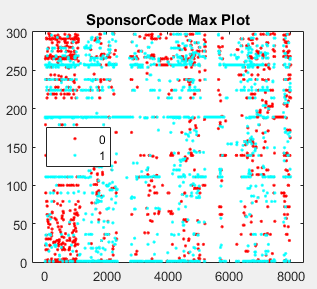
\includegraphics[scale=0.5]{SponsorPlot.png}}
		\fbox{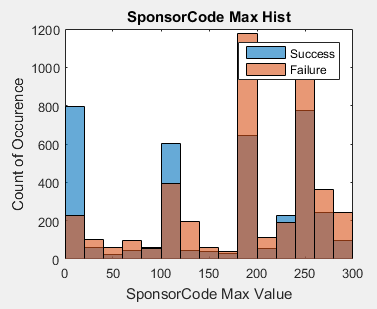
\includegraphics[scale=0.5]{SponsorHist.png}}
	\end{center}
	\caption{Scatter Plot and Histogram for Sponsor Codes.}
\end{figure}

We take an example of Sponsor code for which we plot the data and see a discerning pattern here. We can see that for specific codes, the chances of getting a grant is more.

But we could not find any conclusive pattern in any of the plots and thus, moved on with the classification. Since decision trees doesn't have much problem with the number of dimension we have here. We move ahead with building a decision tree and random forest classifier. For the decision tree we opted for a 5-fold cross validation. The results from the classification models along with the confusion matrices are as listed below:

\begin{figure}[h]
	\begin{center}
		%\framebox[4.0in]{$\;$}
		\fbox{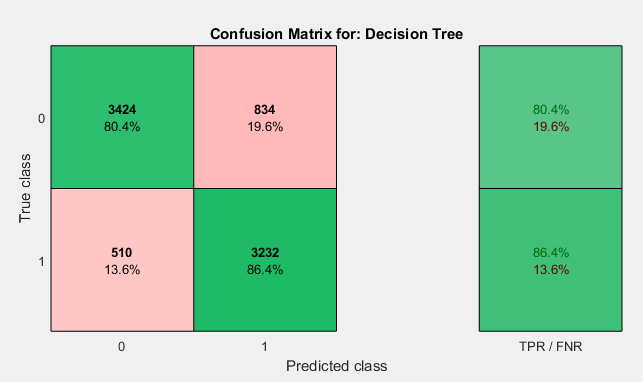
\includegraphics[scale=0.5]{DecisionTreeCM.png}}
	\end{center}
	\caption{Confusion Matrix and TPR/FPR of Simple Decision Tree.}
\end{figure}

\begin{figure}[h]
	\begin{center}
		%\framebox[4.0in]{$\;$}
		\fbox{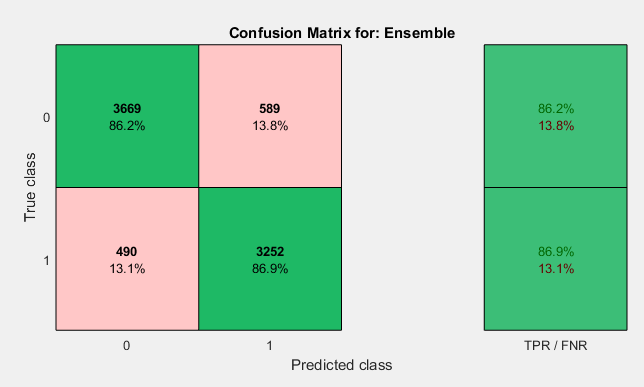
\includegraphics[scale=0.5]{RandomForestCM.png}}
	\end{center}
	\caption{Confusion Matrix and TPR/FPR of Random Forest.}
\end{figure}

In addition, we found the important features which determine the outcome of the application. The data is plotted in . From the plot we can see that features Contract Value(3), Sponsor Code(1), Application Month(14), Grant Category(2) are the most important factors.

\begin{figure}[h]
	\begin{center}
		%\framebox[4.0in]{$\;$}
		\fbox{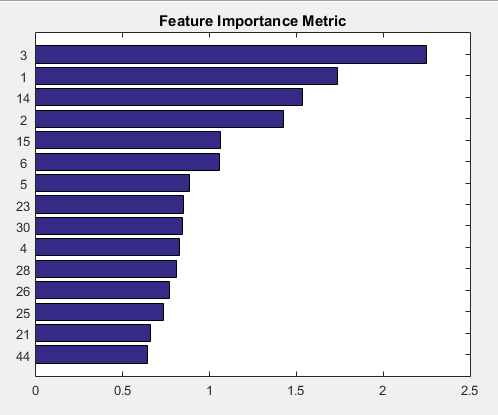
\includegraphics[scale=0.5]{FIM.png}}
	\end{center}
	\caption{Feature Importance Matrix Generated By Random Forest.}
\end{figure}
 


\section{Citations, figures, tables, references}
\label{others}

These instructions apply to everyone, regardless of the formatter being used.

\subsection{Citations within the text}

Citations within the text should be numbered consecutively. The corresponding
number is to appear enclosed in square brackets, such as [1] or [2]-[5]. The
corresponding references are to be listed in the same order at the end of the
paper, in the \textbf{References} section. (Note: the standard
\textsc{Bib\TeX} style \texttt{unsrt} produces this.) As to the format of the
references themselves, any style is acceptable as long as it is used
consistently.

As submission is double blind, refer to your own published work in the 
third person. That is, use ``In the previous work of Jones et al.\ [4]'',
not ``In our previous work [4]''. If you cite your other papers that
are not widely available (e.g.\ a journal paper under review), use
anonymous author names in the citation, e.g.\ an author of the
form ``A.\ Anonymous''. 


\subsection{Footnotes}

Indicate footnotes with a number\footnote{Sample of the first footnote} in the
text. Place the footnotes at the bottom of the page on which they appear.
Precede the footnote with a horizontal rule of 2~inches
(12~picas).\footnote{Sample of the second footnote}

\subsection{Figures}

All artwork must be neat, clean, and legible. Lines should be dark
enough for purposes of reproduction; art work should not be
hand-drawn. The figure number and caption always appear after the
figure. Place one line space before the figure caption, and one line
space after the figure. The figure caption is lower case (except for
first word and proper nouns); figures are numbered consecutively.

Make sure the figure caption does not get separated from the figure.
Leave sufficient space to avoid splitting the figure and figure caption.

You may use color figures. 
However, it is best for the
figure captions and the paper body to make sense if the paper is printed
either in black/white or in color.
\begin{figure}[h]
\begin{center}
%\framebox[4.0in]{$\;$}
\fbox{\rule[-.5cm]{0cm}{4cm} \rule[-.5cm]{4cm}{0cm}}
\end{center}
\caption{Sample figure caption.}
\end{figure}

\subsection{Tables}

All tables must be centered, neat, clean and legible. Do not use hand-drawn
tables. The table number and title always appear before the table. See
Table~\ref{sample-table}.

Place one line space before the table title, one line space after the table
title, and one line space after the table. The table title must be lower case
(except for first word and proper nouns); tables are numbered consecutively.

\begin{table}[t]
\caption{Sample table title}
\label{sample-table}
\begin{center}
\begin{tabular}{ll}
\multicolumn{1}{c}{\bf PART}  &\multicolumn{1}{c}{\bf DESCRIPTION}
\\ \hline \\
Dendrite         &Input terminal \\
Axon             &Output terminal \\
Soma             &Cell body (contains cell nucleus) \\
\end{tabular}
\end{center}
\end{table}

\section{Final instructions}
Do not change any aspects of the formatting parameters in the style files.
In particular, do not modify the width or length of the rectangle the text
should fit into, and do not change font sizes (except perhaps in the
\textbf{References} section; see below). Please note that pages should be
numbered.

\section{Preparing PostScript or PDF files}

Please prepare PostScript or PDF files with paper size ``US Letter'', and
not, for example, ``A4''. The -t
letter option on dvips will produce US Letter files.

Fonts were the main cause of problems in the past years. Your PDF file must
only contain Type 1 or Embedded TrueType fonts. Here are a few instructions
to achieve this.

\begin{itemize}

\item You can check which fonts a PDF files uses.  In Acrobat Reader,
select the menu Files$>$Document Properties$>$Fonts and select Show All Fonts. You can
also use the program \verb+pdffonts+ which comes with \verb+xpdf+ and is
available out-of-the-box on most Linux machines.

\item The IEEE has recommendations for generating PDF files whose fonts
are also acceptable for NIPS. Please see
\url{http://www.emfield.org/icuwb2010/downloads/IEEE-PDF-SpecV32.pdf}

\item LaTeX users:

\begin{itemize}

\item Consider directly generating PDF files using \verb+pdflatex+
(especially if you are a MiKTeX user). 
PDF figures must be substituted for EPS figures, however.

\item Otherwise, please generate your PostScript and PDF files with the following commands:
\begin{verbatim} 
dvips mypaper.dvi -t letter -Ppdf -G0 -o mypaper.ps
ps2pdf mypaper.ps mypaper.pdf
\end{verbatim}

Check that the PDF files only contains Type 1 fonts. 
%For the final version, please send us both the Postscript file and
%the PDF file. 

\item xfig "patterned" shapes are implemented with 
bitmap fonts.  Use "solid" shapes instead. 
\item The \verb+\bbold+ package almost always uses bitmap
fonts.  You can try the equivalent AMS Fonts with command
\begin{verbatim}
\usepackage[psamsfonts]{amssymb}
\end{verbatim}
 or use the following workaround for reals, natural and complex: 
\begin{verbatim}
\newcommand{\RR}{I\!\!R} %real numbers
\newcommand{\Nat}{I\!\!N} %natural numbers 
\newcommand{\CC}{I\!\!\!\!C} %complex numbers
\end{verbatim}

\item Sometimes the problematic fonts are used in figures
included in LaTeX files. The ghostscript program \verb+eps2eps+ is the simplest
way to clean such figures. For black and white figures, slightly better
results can be achieved with program \verb+potrace+.
\end{itemize}
\item MSWord and Windows users (via PDF file):
\begin{itemize}
\item Install the Microsoft Save as PDF Office 2007 Add-in from
\url{http://www.microsoft.com/downloads/details.aspx?displaylang=en\&familyid=4d951911-3e7e-4ae6-b059-a2e79ed87041}
\item Select ``Save or Publish to PDF'' from the Office or File menu
\end{itemize}
\item MSWord and Mac OS X users (via PDF file):
\begin{itemize}
\item From the print menu, click the PDF drop-down box, and select ``Save
as PDF...''
\end{itemize}
\item MSWord and Windows users (via PS file):
\begin{itemize}
\item To create a new printer
on your computer, install the AdobePS printer driver and the Adobe Distiller PPD file from
\url{http://www.adobe.com/support/downloads/detail.jsp?ftpID=204} {\it Note:} You must reboot your PC after installing the
AdobePS driver for it to take effect.
\item To produce the ps file, select ``Print'' from the MS app, choose
the installed AdobePS printer, click on ``Properties'', click on ``Advanced.''
\item Set ``TrueType Font'' to be ``Download as Softfont''
\item Open the ``PostScript Options'' folder
\item Select ``PostScript Output Option'' to be ``Optimize for Portability''
\item Select ``TrueType Font Download Option'' to be ``Outline''
\item Select ``Send PostScript Error Handler'' to be ``No''
\item Click ``OK'' three times, print your file.
\item Now, use Adobe Acrobat Distiller or ps2pdf to create a PDF file from
the PS file. In Acrobat, check the option ``Embed all fonts'' if
applicable.
\end{itemize}

\end{itemize}
If your file contains Type 3 fonts or non embedded TrueType fonts, we will
ask you to fix it. 

\subsection{Margins in LaTeX}
 
Most of the margin problems come from figures positioned by hand using
\verb+\special+ or other commands. We suggest using the command
\verb+\includegraphics+
from the graphicx package. Always specify the figure width as a multiple of
the line width as in the example below using .eps graphics
\begin{verbatim}
   \usepackage[dvips]{graphicx} ... 
   \includegraphics[width=0.8\linewidth]{myfile.eps} 
\end{verbatim}
or % Apr 2009 addition
\begin{verbatim}
   \usepackage[pdftex]{graphicx} ... 
   \includegraphics[width=0.8\linewidth]{myfile.pdf} 
\end{verbatim}
for .pdf graphics. 
See section 4.4 in the graphics bundle documentation (\url{http://www.ctan.org/tex-archive/macros/latex/required/graphics/grfguide.ps}) 
 
A number of width problems arise when LaTeX cannot properly hyphenate a
line. Please give LaTeX hyphenation hints using the \verb+\-+ command.





\begin{thebibliography}{100} % 100 is a random guess of the total number of
	%references
	\bibitem{Top10} Top 10 algorithms in data mining. Knowl. Inf. Syst. 14, 1 (December 2007), 1-37. DOI=http://dx.doi.org/10.1007/s10115-007-0114-2
	\bibitem{OneRow} Efficient “One-Row-per-Subject” Data Mart Construction for Data Mining, Gerhard Svolba, PhD, SAS Austria
	\bibitem{Multi} Reliable Early Classification on Multivariate Time Series with Numerical and Categorical Attributes, Cao, Tru et al.
	\bibitem{HighCard}Daniele Micci-Barreca. 2001. A preprocessing scheme for high-cardinality categorical attributes in classification and prediction problems. SIGKDD Explor. Newsl. 3, 1 (July 2001), 27-32. DOI=http://dx.doi.org/10.1145/507533.
	\bibitem{Matlab}Kaggle
\end{thebibliography}

\end{document}
